\begin{frame}{}
  \centering
  \Large
  \textbf{Partie 1}

  \textbf{Fondamentaux}
\end{frame}

\section{Concepts de base : syntaxe et types}

\begin{frame}[fragile]{Syntaxe}
  
  \begin{itemize}
    \item<+->[\textcolor{white}{a}] La syntaxe de Python repose sur une série d'instructions et des mots clés bien précis
\begin{lstlisting}[language=Python, morekeywords={as, TypeError}, numbers=none]
>>> a = "Hello, world"
>>> print(a)
"Hello, world"
\end{lstlisting}
    \item<+-> \texttt{a} est une \textbf{variable} et "Hello, world" est sa \textbf{valeur}
    \item<+-> la variable \texttt{a} est un objet
    \item<+-> la variable \texttt{a} a un type
\begin{lstlisting}[language=Python, morekeywords={as, TypeError}, numbers=none]
>>> print(type(a))
str
\end{lstlisting}
  \end{itemize}
\end{frame}

\begin{frame}[fragile]{Syntaxe}

  Les noms de variables sont libres à l'exception de certains mots réservés :

\begin{lstlisting}[language=bash, morekeywords={def, list, class, global, else, in}, numbers=none]
def, return, class, global, else, in
\end{lstlisting}

Liste complète \href{https://docs.python.org/3/reference/lexical\_analysis.html\#keywords}{ici}

\begin{block}{Conventions}
  \begin{itemize}
    \item Ne pas mettre de caractère accentués ni de caractère non ASCII et préférer l'anglais
    \item Choisir des noms de variables qui soient compréhensibles
    \item Vous pouvez choisir des noms en plusieurs mots s'il n'est pas trop long, séparer les mots par un ``\_'', ou mettre des majuscules.
  \end{itemize}
\end{block}
\end{frame}

\begin{frame}[fragile]{Syntaxe}

  \begin{itemize}
    \item<+->[\textcolor{white}{a}]La syntaxe de Python repose sur une série d'instructions et des mots clés bien précis.
\begin{lstlisting}[language=Python, morekeywords={as, TypeError}, numbers=none]
>>> a = "Hello, world"
>>> print(a)
"Hello, world"
\end{lstlisting}
    \item<+->[\textcolor{white}{a}]Le même texte aurait pu être affiché d'une façon différente.
\begin{lstlisting}[language=Python, morekeywords={as, TypeError}, numbers=none]
>>> a = "Hello,"
>>> b = "world"
>>> print(a, b)
"Hello, world"
\end{lstlisting}
    \item<+->[\textcolor{white}{a}]Ou encore de cette façon.
\begin{lstlisting}[language=Python, morekeywords={as, TypeError}, numbers=none]
>>> a = "Hello, "
>>> b = "world"
>>> print(a + b)
"Hello, world"
\end{lstlisting}
  \end{itemize}

\end{frame}

\begin{frame}[fragile]{Types de base : types numériques}
  
  \begin{block}{}
    \begin{itemize}
      \item Entier, \texttt{int}
\begin{lstlisting}[language=Python, morekeywords={as, TypeError}, numbers=none]
>>> a = 1
\end{lstlisting}
      \item Flottant, \texttt{float}
\begin{lstlisting}[language=Python, morekeywords={as, TypeError}, numbers=none]
>>> a = 1.1
\end{lstlisting}
      \item Booléen, \texttt{bool}
\begin{lstlisting}[language=Python, morekeywords={as, TypeError}, numbers=none]
>>> a = True
>>> b = False
\end{lstlisting}
    \end{itemize}
  \end{block}
\end{frame}

\begin{frame}[fragile]{Opérations sur les types numériques}
    \underline{Opérations élémentaires :}
    \medskip
\begin{lstlisting}[language=Python, morekeywords={as, TypeError}, numbers=none]
>>> 10 + 4
14
>>> 10 - 4
6
>>> 10 * 4
40
>>> 10 ** 4
10000
>>> 10 / 4
2.5
>>> 10 / float(4)
2.5
>>> 7 // 3
2
>>> 7 % 3
1
\end{lstlisting}
\end{frame}
  
  
\begin{frame}[fragile]{Types de base : types itérables}
  
  \begin{block}{Types itérables, i.e. des séquences}
    \begin{itemize}
      \item Liste, \texttt{list}
\begin{lstlisting}[language=Python, morekeywords={as, TypeError}, numbers=none]
>>> a = [1, 2, 3]
\end{lstlisting}
      \item Tuple, \texttt{tuple}
\begin{lstlisting}[language=Python, morekeywords={as, TypeError}, numbers=none]
>>> a = (1, 2, 3)
\end{lstlisting}
      \item Dictionnaires, \texttt{dict}
\begin{lstlisting}[language=Python, morekeywords={as, TypeError}, numbers=none]
>>> a = {"key1": 1, "key2": 2, "key3": 3}
\end{lstlisting}
    \end{itemize}
  \end{block}
\end{frame}


\section{Structures de contrôle}

\begin{frame}[fragile]{Structures de contrôle}
  \begin{block}{Instruction if, elif, else}
  \medskip  
\begin{lstlisting}[language=Python, morekeywords={True, false}, numbers=none]
>>> if [condition1]:
...     [instructions]
... elif [condition2]:
...     [instructions]
... else:
...     [instructions]
\end{lstlisting}

  \end{block}

  Remarque : \texttt{elif} et \texttt{else} sont optionnels
\end{frame}

\begin{frame}[fragile]{Opérations sur les booléens et comparaisons}

  \underline{Opérations :}

\begin{lstlisting}[language=Python, morekeywords={True, false}, numbers=none]
>>> a = True
>>> b = a and False   # idem que b = a & False
>>> c = not a
>>> d = bool(0)
>>> e = bool(1)
\end{lstlisting}
  
    \underline{Comparaisons :}
    \medskip
\begin{lstlisting}[language=Python, morekeywords={True, false}, numbers=none]
>>> 5 > 3
>>> 5 >= 3
>>> 5 != 3
>>> 5 == 5
>>> 5 > 3 and 6 > 3
>>> 5 > 3 or 5 < 3
>>> not False
>>> False or not False and True
\end{lstlisting}
\end{frame}

\begin{frame}[fragile]{Structures de contrôle}
  \begin{block}{Instruction if, elif, else}
  \medskip  

  Exemple :
  \begin{overprint}
    \onslide<1>
\begin{lstlisting}[language=Python, morekeywords={True, false}, numbers=none]
>>> if i == 0:
...     print("i equals 0")
\end{lstlisting}

    \onslide<2>
\begin{lstlisting}[language=Python, morekeywords={True, false}, numbers=none]
>>> i = 0
>>> condition = i != 0
>>> if not condition:
...     print("i equals 0")
\end{lstlisting}
  \end{overprint}


  \end{block}

  Remarque : \texttt{elif} et \texttt{else} sont optionnels
\end{frame}

\begin{frame}[fragile]{Structures de contrôle}
  Il est possible de définir une variable selon certaines conditions.
\begin{lstlisting}[language=Python, numbers=none]
>>> if not i:
...     a = 1
... else:
...     a = 2
\end{lstlisting}

\begin{lstlisting}[language=Python, numbers=none]
>>> a = 1 if not i else 2
\end{lstlisting}
\end{frame}

\begin{frame}[fragile]{Structures de contrôle}
  \begin{block}{Boucle while}
  \medskip  
\begin{lstlisting}[language=Python, morekeywords={True, false}, numbers=none]
>>> while [condition]:
...     [instructions]
\end{lstlisting}
  \end{block}

    Exemple :
    \begin{overprint}
    \onslide<1>
    
\begin{lstlisting}[language=Python, morekeywords={True, false}, numbers=none]
>>> i = 0
>>> while i < 10:
...     print(i)
...     i += 1
\end{lstlisting}

  \onslide<2>
\begin{lstlisting}[language=Python, morekeywords={True, false}, numbers=none]
>>> i = 0
>>> while i < 10:
...     print(i)
\end{lstlisting}
La boucle ne s'arrêtra que quand l'ordinateur plantera

\end{overprint}
\end{frame}


\section{Fonctions}

\begin{frame}[fragile]{Syntaxe}

  \begin{itemize}
    \item<+->[\textcolor{white}{a}]Précedemment nous avons utilisé print plusieurs fois.
\begin{lstlisting}[language=Python, morekeywords={as, TypeError}, numbers=none]
>>> a = "Hello, world"
>>> print(a)
"Hello, world"
\end{lstlisting}
    \item<+->[\textcolor{white}{a}]Et de façons différentes.
\begin{lstlisting}[language=Python, morekeywords={as, TypeError}, numbers=none]
>>> a = "Hello,"
>>> b = "world"
>>> print(a, b)
"Hello, world"
\end{lstlisting}
    \item<+->[\textcolor{white}{a}]En fait \textbf{print est une fonction avec des arguments}.
\begin{lstlisting}[language=Python, morekeywords={as, TypeError}, numbers=none]
print(*objects, sep=' ', end='\n', file=None, flush=False)
\end{lstlisting}
  \end{itemize}

\end{frame}


\begin{frame}[fragile]{Fonctions}
  %TO DO : fonctions avec ou sans valeurs par défaut
  %args, kwargs
  Mots clés pour définir une fonction : \texttt{def} et \texttt{return}

  \begin{overprint}
    
    \onslide<1>
\begin{lstlisting}[language=Python, morekeywords={}, numbers=none]
>>> def fct(a, b, c):
...     # a, b et c sont des arguments positionnels
...     d = (a + b) * c
...     return d

>>> fct(1, 2, 3)
\end{lstlisting}

  \onslide<2>
\begin{lstlisting}[language=Python, morekeywords={}, numbers=none]
>>> def fct(a=1, b=1, c=1):
...     # a, b et c sont des arguments nommes
...     d = (a + b) * c
...     return d

>>> fct()
\end{lstlisting}

  \onslide<3>
\begin{lstlisting}[language=Python, morekeywords={}, numbers=none]
>>> def fct(a, b, c=None):
...     # a et b sont des arguments positionnels, c est un argument nomme
...     if not c:
...         d = a + b
...     else:
...         d = (a + b) * c
...     return d

>>> fct(1, 2)
\end{lstlisting}
    
  
  \end{overprint}

    \begin{itemize}
      \item \texttt{fct} est le nom de notre fonction
      \item a, b et c sont les arguments (\textbf{nommés} ou \textbf{positionnels})
      \item d est le retour de la fonction
    \end{itemize}

\end{frame}
  

% \begin{frame}[fragile]{Fonction lambda}
%   Une autre manière de définir une fonction :
% \begin{lstlisting}[language=Python, morekeywords={}, numbers=none]
% >>> def sum(a, b):
% ...     return a + b
% \end{lstlisting}

% Avec \texttt{lambda} :
% \begin{lstlisting}[language=Python, morekeywords={}, numbers=none]
% >>> sum = lambda a, b: a + b
% \end{lstlisting}
    
% \end{frame}


% \begin{frame}[fragile]{Fonction lambda}
%   Une autre manière de définir une fonction :
% \begin{lstlisting}[language=Python, morekeywords={}, numbers=none]
% >>> def fct(a, b, c=None):
% ...     if not c:
% ...         d = a + b
% ...     else:
% ...         d = (a + b) * c
% ...     return d
% \end{lstlisting}

% Avec \texttt{lambda} :
% \begin{lstlisting}[language=Python, morekeywords={}, numbers=none]
% >>> ???
% \end{lstlisting}
% \end{frame}







\section{Listes}
\begin{frame}[fragile]{Listes}
Une liste est un contenant permettant de concaténer différent objects :
  \begin{lstlisting}[language=Python, morekeywords={as, TypeError}, numbers=none]
>>> my_list = [True, 2, "3", 4]
  \end{lstlisting}

Il n'y a pas de restrictions sur les objects contenus dans les listes, ils
peuvent être de différents types et même être des listes !
\end{frame}

\begin{frame}[fragile]{Boucler sur une liste}

  \onslide<1->

\begin{lstlisting}[language=Python, morekeywords={True, false}, numbers=none]
>>> for item in my_list:
...     print(item)
\end{lstlisting}
    
  \onslide<2>
Avec le mot clé \texttt{enumerate}
\begin{lstlisting}[language=Python, morekeywords={True, false}, numbers=none]
>>> for i, item in enumerate(my_list):
...     print(i, item)
\end{lstlisting}
\end{frame}

\begin{frame}[fragile]{Listes}

  Une liste est une séquence d'objets potentiellement de types différents :
\begin{lstlisting}[language=Python, morekeywords={True, false}, numbers=none]
>>> my_list = [True, 2, "3", 4]
\end{lstlisting}
  
  Accès par indice :
  \begin{center}
  \texttt{my\_list[start:stop:step]}
  \end{center}

  Les indices commencent à 0 et peuvent être négatifs
\end{frame}

\begin{frame}[fragile]{Listes}

  Par exemple :
\begin{lstlisting}[language=Python, morekeywords={True, false}, numbers=none]
>>> my_list[0]
True

>>> my_list[0:2]
[True, 2]

>>> my_list[0:4:2]
[True, "3"]

>>> my_list[-1]
4
>>> my_list[::-1]
[4, "3", 2, True]

\end{lstlisting}

\end{frame}


\begin{frame}[fragile]{Listes}

  Autres opérations utiles :
\begin{lstlisting}[language=Python, morekeywords={True, false}, numbers=none]
>>> print(2 in my_list)
True

>>> list(range(4))
[0, 1, 2, 3]

>>> my_list + [10, 11]
[True, 2, "3", 4, 10, 11]

>>> my_list * 2
[True, 2, "3", 4, True, 2, "3", 4]
\end{lstlisting}

\end{frame}



\begin{frame}{Opérations sur les listes}

  \begin{itemize}
    \item Remplacer un élément
    \item Remplacer une sous-séquence (slicing)
    \item Supprimer des éléments
    \item Concaténer deux listes
    \item Répéter les élements d'une liste
    \item Ajout d'un élement en fin de liste
  \end{itemize}
  
\end{frame}

\begin{frame}[fragile]{Méthodes et attributs d'une liste}
  Méthodes :
  \begin{columns}[T]
    \begin{column}{.48\textwidth}
      \begin{itemize}
        \item \texttt{append}: ajout d'un élément.
        \item \texttt{clear}: vider la liste.
        \item \texttt{copy}: copier la liste.
        \item \texttt{count}: nombre de fois où l'élément apparaît.
        \item \texttt{index}: position où l'élément apparaît.
        \item \texttt{extend}: ajout d'une liste.
      \end{itemize}
    \end{column}

    \begin{column}{.48\textwidth}
      \begin{itemize}
        \item \texttt{insert}: mettre un object à la position i.
        \item \texttt{pop}: supprimer l'élément à la position i.
        \item \texttt{remove}: supprimer l'élément i.
        \item \texttt{reverse}: inverser la liste.
        \item \texttt{sort}: trier la liste.
      \end{itemize}
    \end{column}
  \end{columns}

  \bigskip

\begin{lstlisting}[language=Python, numbers=none]
my_list = [1, 2, 3]
my_list.<nom de la methode>(<arguments>)
my_list.append(1)
\end{lstlisting}
\end{frame}


\begin{frame}[fragile]{Compréhension de liste}

Exemple : calculer le carré de chaque élément d'une liste d'entiers

\begin{overprint}
  

\onslide<1>
\begin{lstlisting}[language=Python, morekeywords={True, false}, numbers=none]
>>> my_list = [1, 2, 3, 4]
>>>
>>> 

\end{lstlisting}



\onslide<2->
\begin{lstlisting}[language=Python, morekeywords={True, false}, numbers=none]
>>> my_list = [1, 2, 3, 4]
>>> new_list = []
>>> for item in my_list:
...     new_list.append(item**2)
\end{lstlisting}

\end{overprint}


\onslide<3>
Via une liste de compréhension :
\begin{lstlisting}[language=Python, morekeywords={True, false}, numbers=none]
>>> my_list = [1, 2, 3, 4]
>>> new_list = [item**2 for item in my_list]
\end{lstlisting}

Plus rapide, plus lisible !
\end{frame}






\section{Chaînes de caractères}


\begin{frame}[fragile]{Chaînes de caractères}

  \begin{block}{Plusieurs manières d'écrire}
    \medskip
\begin{lstlisting}[language=Python, numbers=none]
>>> s = "une chaine de caracteres"
>>> s = 'une chaine de caracteres'
>>> s = """une chaine 
de caracteres"""
\end{lstlisting}
  \end{block}

  \begin{block}{Accès aux éléments}
  \medskip
\begin{lstlisting}[language=Python, numbers=none]
>>> s = "python"
>>> print(s[0])
"p"
>>> print(s[1:3])
"yt"
>>> print(s[1:6:2])
"yhn"\end{lstlisting}
\end{block}

\end{frame}








\begin{frame}[fragile]{Chaînes de caractères}

  \begin{block}{Boucler sur un chaine de caractères}
    \medskip
\begin{lstlisting}[language=Python, numbers=none]
>>> for item in "python":
...     print(item)
\end{lstlisting}
  \end{block}

  \begin{block}{Concaténer plusieurs chaînes de caractères}
  \medskip
\begin{lstlisting}[language=Python, numbers=none]
>>> s = "une chaine" + "de" + "caracteres"
>>> print(s)
"une chainedecaracteres"
\end{lstlisting}
  \end{block}

\end{frame}


\begin{frame}[fragile]{f-strings}

  \begin{block}{Formatter une chaîne de caractères}
    \medskip
\begin{lstlisting}[language=Python, numbers=none]
>>> pi = 3.14159
>>> print(f"pi = {pi}")
pi = 3.14159
>>> print(f"pi = {pi:.2f}")
pi = 3.14
>>> print(f"pi = {pi:8.2f}")
pi =     3.14
\end{lstlisting}
  \end{block}
\end{frame}

\begin{frame}[fragile]{f-strings}

  \begin{block}{Formatter une chaîne de caractères}
    \medskip
\begin{lstlisting}[language=Python, numbers=none]
coordinates = [(53.123, 26.589), (20.720, 70.447), (80.294, 50.382)]

print(f"{'Index':>10} | {'Latitude':<9} | {'Longitude':<9}")
for i, (lat, lon) in enumerate(coordinates):
    print(f"{i:10} | {lat:<9.3f} | {lon:<9.3f}")

\end{lstlisting}
Outputs :
\begin{lstlisting}[language=Python, numbers=none]

     Index | Latitude  | Longitude
         0 | 53.123    | 26.589   
         1 | 20.720    | 70.447   
         2 | 80.294    | 50.382  

\end{lstlisting}
  \end{block}
\end{frame}



\begin{frame}{Chaînes de caractères}
  Quelques méthodes utiles :
  \begin{itemize}
    \item \texttt{lower}
    \item \texttt{upper}
    \item \texttt{join}
    \item \texttt{replace}
    \item \texttt{split}
  \end{itemize}
  
\end{frame}


\begin{frame}[fragile]{Chaînes de caractères}

  \onslide<1->
\begin{lstlisting}[language=Python, numbers=none]
>>> a = "    Hello, etienne guevel   "
>>> a = a.strip()
>>> a = a.title()
>>> print(a)
Hello, Etienne Guevel
\end{lstlisting}
    
  \onslide<2>
Les méthodes peuvent être chaînées !
\begin{lstlisting}[language=Python, numbers=none]
>>> a = "    Hello, etienne guevel   "
>>> a = a.strip().title()
>>> print(a)
Hello, Etienne Guevel
\end{lstlisting}
\end{frame}

\section{Typage}


\begin{frame}[fragile]{Langage dynamiquement typé}

  \begin{block}{Dynamique vs Statique}
  \medskip
    \begin{itemize}
      \item Dynamique : le type est déterminé au \textbf{moment de l'exécution} et peut \textbf{changer}
      \item Statique : le type est fixé en début de programme
    \end{itemize}
  \end{block}

  \begin{block}{Inférence de type}
  \medskip
  Python détermine automatiquement le type d'une variable
  \end{block}

\begin{lstlisting}[language=Python, morekeywords={as, TypeError}, numbers=none]
>>> a = 1
>>> print(type(a))
int
>>> a = "hello"
>>> print(type(a))
str
\end{lstlisting}
\end{frame}




\begin{frame}[fragile]{Typage fort}
  \medskip
    \begin{itemize}
      \item le type d'un objet est déterminé par l'ensemble de ses caractéristiques % on se concentre sur les caractéristiques des objets plutôt que du type lui même
      \item En particulier, une même opération peut fonctionner sur \textbf{objets de type différents}, si tant est que les opérations soient valables
    \end{itemize}

\begin{lstlisting}[language=Python, morekeywords={as}, numbers=none]
>>> 5 + 4
9
>>> "titi" + "toto"
"tititoto"
\end{lstlisting}

\end{frame}

\begin{frame}[fragile]{Typage fort}
    \begin{block}{Corolaire}
      \medskip
      Python \textbf{interdit} des opérations ayant peu de sens et \textbf{ne cherche pas à convertir} lui même.

      Par exemple :
      \begin{itemize}
        \item \textbf{On ne peut pas} \textcolor{red}{ajouter} une chaîne de caractère et un entier
        \item \textbf{On peut} \textcolor{red}{multiplier} une chaîne de caractère et un entier
      \end{itemize}

    \end{block}

\begin{lstlisting}[language=Python, morekeywords={as, TypeError}, numbers=none]
>>> "titi" * 2
"titititi"

>>> "titi" + 2
TypeError: can only concatenate str (not "int") to str
\end{lstlisting}

\end{frame}

\section{Tuples}

\begin{frame}[fragile]{Tuples}

  Un tuple est une séquence immutable d'objets potentiellement de types différents :
\begin{lstlisting}[language=Python, morekeywords={True, false}, numbers=none]
>>> my_tuple = (True, 2, "3", 4)
>>> my_tuple = (1,)
\end{lstlisting}
  
  Accès par indice :
\begin{lstlisting}[language=Python, morekeywords={True, false}, numbers=none]
>>> my_tuple[0]
True
\end{lstlisting}
  % ici j'explique au tableau : len, append, slicing
\end{frame}

\begin{frame}{Comparaison avec les listes}

  \begin{itemize}
    \item \sout{Remplacer un élément}
    \item \sout{Remplacer une sous-séquence (slicing)}
    \item \sout{Supprimer des éléments}
    \item Concaténer deux tuples
    \item Répéter les éléments d'un tuple
    \item \sout{Ajout d'un élément en fin de tuple}
  \end{itemize}
  
\end{frame}


\begin{frame}[fragile]{Boucler sur un tuple}

  \onslide<1->

\begin{lstlisting}[language=Python, morekeywords={True, false}, numbers=none]
>>> for item in my_tuple:
...     print(item)
\end{lstlisting}
    
  \onslide<2->
Avec le mot clé \texttt{range}
\begin{lstlisting}[language=Python, morekeywords={True, false}, numbers=none]
>>> for i in range(len(my_tuple)):
...     print(my_tuple[i])
\end{lstlisting}
    
  \onslide<3>
Avec le mot clé \texttt{enumerate}
\begin{lstlisting}[language=Python, morekeywords={True, false}, numbers=none]
>>> for i, item in enumerate(my_tuple):
...     print(i, item)
\end{lstlisting}
\end{frame}


\section{Mutabilité}


\begin{frame}{Mutable vs immutable}

  \begin{block}{Objet mutable}
    \medskip
    Un objet mutable \textcolor{red}{peut être modifié} après sa création
    \begin{itemize}
      \item list
      \item dict
      \item set
    \end{itemize}
  \end{block}


  \begin{block}{Objet immutable}
    \medskip
    Un objet immutable \textcolor{red}{ne peut être modifié} après sa création
    \begin{itemize}
      \item int, float, bool
      \item str
      \item tuple
      \item byte
    \end{itemize}
  \end{block}

\end{frame}


\begin{frame}[fragile]{Mutable vs immutable}
  
  \begin{block}{Immutabilité : modification d'un entier}
    \medskip
\begin{lstlisting}[language=Python, morekeywords={as, True, False}, numbers=none]
>>> a = 1
>>> b = a
>>> id(a)
xxxxxxx560
>>> id(b)
xxxxxxx560
>>> a += 1
>>> id(a)
xxxxxxx592
>>> id(b)
xxxxxxx560

\end{lstlisting}
  \end{block}

\onslide<2>
\begin{center}
  \textcolor{red}{\textbf{Copie implicite}}
\end{center}

% \onslide<3>
% \begin{center}
%   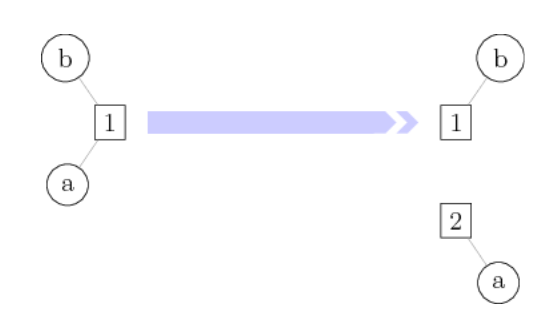
\includegraphics[scale=0.25]{img/image.png}
% \end{center}
\end{frame}



\begin{frame}[fragile]{Mutable vs immutable}
  
  \begin{block}{Mutabilité : modification d'une liste}
    \medskip
\begin{lstlisting}[language=Python, morekeywords={as, True, False}, numbers=none]
>>> a = [1, 2]
>>> id(a)
xxxxxxx328
>>> a[0] += 1
>>> id(a)
xxxxxxx328
\end{lstlisting}
  \end{block}

  \textcolor{white}{Que se passe-t-il ici ?}
  \begin{center}
    \textcolor{white}{\textbf{Copie implicite}}
  \end{center}
\end{frame}








\begin{frame}[fragile]{Mutable vs immutable}
    \begin{block}{Autre exemple, \texttt{int}}
      \medskip
\begin{lstlisting}[language=Python, morekeywords={as, True, False}, numbers=none]
>>> a = 1
>>> b = a
>>> b is a
True
>>> b += 1
>>> b
2


>>> b is a
False
\end{lstlisting}
    \end{block}
\end{frame}


\begin{frame}[fragile]{Mutable vs immutable}

    \begin{block}{Autre exemple, \texttt{list}}
      \medskip
\begin{lstlisting}[language=Python, morekeywords={as, True}, numbers=none]
>>> a = [1, 2]
>>> b = a
>>> b is a
True
>>> b[0] += 1
>>> b
[2, 2]
>>> a
[2, 2]
>>> b is a
True
\end{lstlisting}
    \end{block}
\end{frame}



\begin{frame}{En bref}
  \begin{block}{}
    \medskip
    \begin{itemize}
      \item Python gère les objets mutables et immutables différemment
      \item Les objets mutables sont très intéressants si on a besoin de changer leur structures (taille, type, etc.) mais cela peut être dangereux
      \item Les objets immutables sont plus rapides d'accès
      \item Les objets immutables doivent être préférés si on veux que l'objet reste le même tout au long de l'exécution
      \item Modifier un objet immutable est plus couteux car il nécessite une copie (explicite ou non)
    \end{itemize}
  \end{block}
\end{frame}





\section{Dictionnaires}

\begin{frame}[fragile]{Dictionnaires}
  Un dictionnaire fonctionne avec le paradigme clé / valeur

\begin{lstlisting}[language=Python, numbers=none]
>>> Larousse["python"]
Serpent monstrueux de la mythologie grecque, qui rendait ses 
oracles a Delphes.
Il fut tue par Apollon qui etablit a Delphes son propre 
oracle.
\end{lstlisting}

\end{frame}

\begin{frame}[fragile]{Dictionnaires}
  Un dictionnaire est une séquence mutable selon le paradigme clé/valeurs :
\begin{lstlisting}[language=Python, morekeywords={True, false}, numbers=none]
>>> my_dict = {"key1": 1, "key2": 2}
>>> my_dict = dict(key1=1, key2=2)
\end{lstlisting}
  
  Accès par clé :
  \onslide<1->
\begin{lstlisting}[language=Python, morekeywords={True, false}, numbers=none]
>>> my_dict["key1"]
1
>>> my_dict.get("key1")
1
\end{lstlisting}

\onslide<2>
Que se passe-t-il si la clé n'existe pas ?
\begin{lstlisting}[language=Python, morekeywords={True, false}, numbers=none]
>>> my_dict["key3"]
?
>>> my_dict.get("key3")
?
\end{lstlisting}
  
\end{frame}




\begin{frame}[fragile]{Dictionnaires}

Ajouter un élément :
\onslide<1->
\begin{lstlisting}[language=Python, morekeywords={True, false}, numbers=none]
>>> my_dict["new_key"] = new_value
\end{lstlisting}

\onslide<2->
\begin{block}{Utiliser la méthode \texttt{update}}
\begin{lstlisting}[language=Python, morekeywords={True, false}, numbers=none]
>>> my_dict.update({"new_key": new_value})
>>> my_dict |= {"other_key": other_value} #since python 3.9
>>> my_dict["new_key"]
new_value
\end{lstlisting}


\end{block}
\end{frame}



\begin{frame}{Opérations sur les dictionnaires}

  \begin{columns}[T]
    \begin{column}{.48\textwidth}
      \begin{block}{Opérations}
        \medskip
        \begin{itemize}
          \item Ajouter un élément
          \item Remplacer un élément
          \item Supprimer des éléments
          \item Concaténer deux dictionnaires
        \end{itemize}
      \end{block}
    \end{column}

    \begin{column}{.48\textwidth}
      \begin{block}{Méthodes associées}
        \medskip
        \begin{itemize}
          \item \texttt{get}
          \item \texttt{keys}
          \item \texttt{values}
          \item \texttt{items}
          \item \texttt{clear}
          \item \texttt{pop}
          \item \texttt{update}
        \end{itemize}
      \end{block}
    \end{column}
  \end{columns}
  
\end{frame}



\begin{frame}[fragile]{Boucler sur un dictionnaire}
  \onslide<1->
\begin{lstlisting}[language=Python, morekeywords={True, false}, numbers=none]
>>> for key in my_dict:
...     print(key, my_dict[key])
\end{lstlisting}
    
  \onslide<2->
\begin{lstlisting}[language=Python, morekeywords={True, false}, numbers=none]
>>> for value in my_dict.values():
...     print(value)
\end{lstlisting}
        
  \onslide<3>
\begin{lstlisting}[language=Python, morekeywords={True, false}, numbers=none]
>>> for key, value in my_dict.items():
...     print(key, value)
\end{lstlisting}
\end{frame}



\section{Ensembles}

\begin{frame}[fragile]{Ensemble}

  Un ensemble est une séquence \textbf{mutable} contenant des éléments \textbf{ordonnés} et \textbf{uniques}. Un ensemble vide est créé par \texttt{set()}.

  \begin{lstlisting}[language=Python, morekeywords={True, false}, numbers=none]
>>> a = {1, 2, 3, 3, 3, 3}
>>> print(a)
{1, 2, 3}
\end{lstlisting}

  Intérêt des ensembles :
  \begin{itemize}
    \item Tests d'appartenance d'un élément à une séquence
    \item Suppression de doublons
  \end{itemize}

\end{frame}

\begin{frame}[fragile]{Ensemble}
Des opérations sont possibles sur les sets :
\begin{lstlisting}[language=Python, morekeywords={&, |, -, ^}, numbers=none]
>>> french_fruits = {"apple", "pear", "banana", "peach"}
>>> american_fruits = {"banana", "peach", "pineapple", "avocado"}
>>> french_fruits & american_fruits
{"banana", "peach"}
>>> french_fruits | american_fruits
{"apple", "pear", "banana", "peach", "pineapple", "avocado"}
>>> french_fruits - american_fruits
{"apple", "pear"}
>>> french_fruits ^ american_fruits
{"apple", "pear", "pineapple", "avocado"}
\end{lstlisting}

\end{frame}

\section{Unpacking}

\begin{frame}[fragile]{Unpacking}

  \onslide<1->
  \begin{block}{Unpacking}
    \medskip
\begin{lstlisting}[language=Python, morekeywords={as, True}, numbers=none]
>>> a, b = [1, 2]
>>> print(a, b)
1 2
\end{lstlisting}
  \end{block}

  \onslide<2->
  \begin{block}{Unpacking plus complexe}
    \medskip
\begin{lstlisting}[language=Python, morekeywords={as, True}, numbers=none]
>>> name, (taille, poids) = ["Antoine", (1.75, 90)]
>>> print(name, taille, poids)
Antoine 1.75 90
\end{lstlisting}
  \end{block}


  \onslide<3->
  \begin{block}{Unpacking avec une taille inconnue}
    \medskip
\begin{lstlisting}[language=Python, morekeywords={as, True}, numbers=none]
>>> start, *_, end = list(range(10))
>>> print(start, end)
0 9
\end{lstlisting}
  \end{block}
\end{frame}



\section{Portée des variables}

\begin{frame}[fragile]{Portée des variables}
  
  Comme dans les autres langages, il existe deux types de variables en python :
  \begin{itemize}
    \item locales : des variables définies dans une fonction
    \item globales : des variables définies en dehors des fonctions
  \end{itemize}  

  \begin{overprint}
    \onslide<1>
\begin{lstlisting}[language=Python, morekeywords={as, True}, numbers=none]
>>> val = 0
>>> def sum(a, b):
... 
... 
...     val = a + b
...     return val

>>> sum(1, 2)
???


>>> print(val)
???   
\end{lstlisting}

  \onslide<2>
\begin{lstlisting}[language=Python, morekeywords={as, True}, numbers=none]
>>> val = 0
>>> def sum(a, b):
... 
... 
...     val = a + b
...     return val

>>> sum(1, 2)
3


>>> print(val)
0
\end{lstlisting}

\onslide<3>
\begin{lstlisting}[language=Python, morekeywords={as, True}, numbers=none]
>>> val = 0
>>> def sum(a, b):
...
...     val += 1
...     total_sum = a + b + val
...     return total_sum

>>> sum(1, 2)
UnboundLocalError: local variable "val" referenced before assignment

>>> print(val)
0
\end{lstlisting}


\onslide<4>
\begin{lstlisting}[language=Python, morekeywords={as, True}, numbers=none]
>>> val = 0
>>> def sum(a, b):
...     global val
...     val += 1
...     total_sum = a + b + val
...     return total_sum

>>> sum(1, 2)
4


>>> print(val)
1
\end{lstlisting}


  \end{overprint}
\end{frame}



\section{Modules et imports}

\begin{frame}{Modules et imports}
  
  \begin{block}{Définition}    
    \medskip
    Un module est un fichier python contenant un ensemble d'instructions (fonctions, classes, etc.)

    Un module peut être 
    \begin{itemize}
      \item <+-> Dans une bibliothèque standard de Python (exemple: \texttt{random}).
      \item <+-> Inclus dans un package ou une librairie installée (exemple: \texttt{numpy}).
      \item <+-> Créé localement, par exemple un fichier \texttt{mon\_module.py}
    \end{itemize}
  \end{block}

  \onslide<4>
  \begin{exampleblock}{Permet}
    \medskip
    \begin{enumerate}
    \item Utiliser les fonctionnalités d'un module dans un autre
    \item Structurer un programme python en plusieurs fichiers (implémentation \textbf{modulaire})
    \item Utiliser des packages open-source
  \end{enumerate}
\end{exampleblock}
  
\end{frame}

\begin{frame}[fragile]{Modules et imports}

  \begin{block}{Exemple : \texttt{random}} 
  \onslide<1->
\begin{lstlisting}[language=Python, numbers=none]
>>> import random
>>> random.randint(1, 10)
4
>>> random.choice(["apple", "banana", "cherry"])
"banana"
\end{lstlisting}
  \onslide<2->
  Utilisation de \texttt{from} pour importer des fonctions spécifiques:
  \begin{lstlisting}[language=Python, numbers=none]
>>> from random import randint, choice
>>> randint(1, 10)
4
>>> choice(["apple", "banana", "cherry"])
"banana"
\end{lstlisting}
  \onslide<3>
  Autres modules : collections, math, copy, typing, etc.
  \end{block}

\end{frame}

\begin{frame}[fragile]{Installation de modules}

  \begin{block}{Installation de modules}
    \medskip
    \begin{itemize}
      \item Utiliser un gestionnaire de paquets (pip, conda, etc.)
      \item Exemple: \texttt{pip install numpy}
      \item Utiliser Anaconda navigator
    \end{itemize}
  \end{block}


\begin{block}{Utilisation des modules importés}
  \begin{lstlisting}[language=Python, numbers=none]
  # On peut importer un module avec un alias
  >>> import numpy as np
  >>> np.sqrt([1, 2, 3])
  array([1.        , 1.41421356, 1.73205081])
  >>> from numpy import sqrt as square_root
\end{lstlisting}
\end{block}

\end{frame}


\begin{frame}[fragile]{Modules et imports}
  \begin{block}{Exemple : \texttt{my\_module.py}} 
    \medskip
\begin{lstlisting}[language=Python, numbers=none]
def prod(a, b):
    return a * b

def add(a, b):
    return a + b
\end{lstlisting}
  \end{block}
  \begin{overprint}


  \onslide<2>
\begin{lstlisting}[language=Python, numbers=none]
>>> import my_module
>>> my_module.add(1, 2)
3
>>> my_module.prod(1, 2)
2
\end{lstlisting}

\onslide<3>
\begin{lstlisting}[language=Python, morekeywords={as}, numbers=none]
>>> import my_module as mod
>>> mod.add(1, 2)
3
>>> mod.prod(1, 2)
2
\end{lstlisting}


  \onslide<4>
\begin{lstlisting}[language=Python, morekeywords={NameError}, numbers=none]
>>> from my_module import add
>>> add(1, 2)
3
>>> prod(1, 2)
NameError: name "prod" is not defined
\end{lstlisting}

  \onslide<5>
\begin{lstlisting}[language=Python, morekeywords={NameError}, numbers=none]
>>> from my_module import add, prod
>>> add(1, 2)
3
>>> prod(1, 2)
2
\end{lstlisting}

  \onslide<6>
\begin{lstlisting}[language=Python, numbers=none]
>>> from my_module import *    # NE SURTOUT PAS UTILISER
>>> add(1, 2)
3
>>> prod(1, 2)
2
\end{lstlisting}

\end{overprint}

\end{frame}



\begin{frame}[fragile]{Modules et imports}

  \begin{block}{Pourquoi proscrire l'utilisation de \texttt{import *} ?}
  \medskip

  Exemple : la fonction \texttt{sqrt} existe dans plusieurs libraries :
  \begin{itemize}
      \item Dans \texttt{math} : calcule la racine carré pour un scalaire
      \item Dans \texttt{numpy} : calcule la racine carré pour un scalaire ou pour chaque élément d'un tableau
  \end{itemize}

\begin{lstlisting}[language=Python, morekeywords={TypeError}, numbers=none]
>>> from numpy import *
>>> from math import *
>>> print(sqrt([1, 2, 3]))
TypeError: must be real number, not list
\end{lstlisting}
  
  \end{block}
\end{frame}

\begin{frame}[fragile]{Structurer un programme}

  \begin{block}{Structure en plusieurs fichiers}
    \begin{itemize}
      \item Un ou plusieurs modules contenant les fonctionnalités implémentées
      \item Un programme principal
    \end{itemize}
  \end{block}

\bigskip

\begin{lstlisting}[numbers=none]
my_project/
  - module1.py
  - module2.py
  - main.py
\end{lstlisting}
\end{frame}



\begin{frame}[fragile]{Structurer un programme}

  \texttt{module1.py}
\begin{lstlisting}[language=python, numbers=none]
import math
import sys

def prod(a, b):
    return a * b

def add(a, b):
    return a + b
\end{lstlisting} 

\texttt{main.py}

\begin{lstlisting}[language=python, numbers=none]
from module1 import add, prod
print(add(1, 2))
print(prod(1, 2))
\end{lstlisting} 
  

\end{frame}
